\subsubsection{Caso d'uso UC8.1.3.3: Creazione esercizi di riempimento degli spazi vuoti}
	\label{UC8.1.3.3}
	\begin{figure}[h]
		\centering
			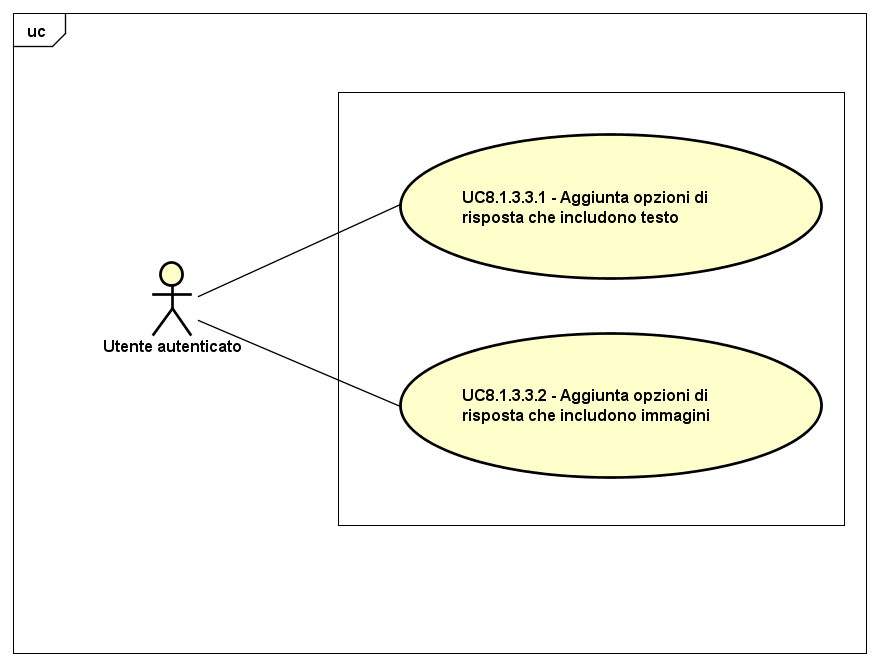
\includegraphics[scale=0.45,keepaspectratio]{UML/UC8_1_3_3.png}
		\caption{UC8.1.3.3: Creazione esercizi di riempimento degli spazi vuoti}
	\end{figure}
	\FloatBarrier
	\begin{itemize}
		\item
			\textbf{Attori}: utente autenticato, utente autenticato pro;
		\item		
			\textbf{Descrizione}: l'attore può creare esercizi di riempimento degli spazi vuoti;
		\item
			\textbf{Precondizione}: l'attore ha selezionato la seguente funzionalità; 
		\item
			\textbf{Postcondizione}: l'attore ha creato un esercizio di riempimento degli spazi vuoti;
		\item
			\textbf{Scenario principale}:
	       		\begin{enumerate}
	       			\item
	       			L'attore può compilare il campo dati destinato alla scrittura del testo dell'esercizio (UC8.1.3.3.1);
	       			\item
	       			L'attore può indicare le parole che saranno sostituite con degli spazi vuoti dal sistema (UC8.1.3.3.2).
	 			\end{enumerate}
	\end{itemize}
	
\subsubsection{Caso d'uso UC8.1.3.3.1: Scrittura testo dell'esercizio}
	\begin{itemize}
		\item
			\textbf{Attori}: utente autenticato, utente autenticato pro;
		\item		
			\textbf{Descrizione}: l'attore può inserire il testo dell'esercizio di riempimento;
		\item
			\textbf{Precondizione}: l'attore può creare un esercizio di riempimento degli spazi vuoti; 
		\item
			\textbf{Postcondizione}: l'attore ha compilato il campo dati dedicato alla scrittura del testo dell'esercizio di riempimento;
		\item
			\textbf{Scenario principale}: l'attore compila il campo dati dedicato alla scrittura del testo dell'esercizio di riempimento.
	\end{itemize}


\subsubsection{Caso d'uso UC8.1.3.3.2: Indicazione parole da oscurare}
	\begin{itemize}
		\item
			\textbf{Attori}: utente autenticato, utente autenticato pro;
		\item		
			\textbf{Descrizione}: l'attore può indicare le parole che saranno sostituite con degli spazi vuoti;
		\item
			\textbf{Precondizione}: l'attore ha inserito il testo dell'esercizio; 
		\item
			\textbf{Postcondizione}: l'attore ha indicato le parole che saranno sostituite con degli spazi vuoti;
		\item
			\textbf{Scenario principale}: l'attore indica le parole che verranno oscurate dal sistema.
	\end{itemize}